%! Author = aybehrouz


\section{Introduction}\label{sec:introduction}

The Argennon\footnote{The classical pronunciation should be used:\textipa{/Ar"gen.non/}} Smart Contract Execution
Environment (AscEE) is an abstract execution environment for executing Argennon smarts contracts (a.k.a\ applications).
An Argennon application essentially is a http server whose state is kept in the Argennon blockchain and
its logic is described using an Argennon Standard Representation (ASR).

An Argennon Standard Representation (ASR) is a programming language for describing argennon applications, optimized
for the architecture and requirements of the Argennon platform.
Argennon supports two standard representations, one is a high level text based language which needs
costly compilation before being executed on a hardware machine. The other one is a low level binary representation which
usually can be executed, with minimal pre-processing, by a JIT compiler or an emulator. The high level
language is intended for preserving high level information of applications logic to facilitate
platform specific compiler optimization at host nodes. On the other hand, the low level language enables efficient
execution of applications that are not frequently used.

The state of an Argennon application is stored in byte addressable finite arrays of memory called
\emph{heap chunks}. An application can have several heap chunks with different sizes, and can remove or
resize its heap chunks or allocate new chunks. Every chunk belongs to exactly one application and can only be modified
by its owner. In addition to heap chunk, every application also has an amount of non-persistent local memory for
storing temporary data.

The Argennon Smart Contract Execution Environment can be seen as a machine for executing http requests, producing
their http response and updating related heap
chunks. The AscEE executes requests sequentially \footnote{Actually requests are executed in parallel but by
performing data dependency analysis the result is guaranteed to be identical with sequential execution of
requests.} and each request has a separate \emph{execution session}. Execution sessions are separate sessions of
executing smart contract's code by the Argennon Smart Contract Execution Environment. The state of an execution
session will be
destroyed at the end of the session and only the state of heap chunks is preserved. If a session fails and does not
complete normally, it will not have any effect on the state of heap chunks.

During an execution session an application can make http requests to other applications. Those requests will not start
a new execution session and will be executed within the current session. In AscEE making a http request is similar to
a function invocation, because of that, we sometimes refer to it as an application
call.

The AscEE is designed based on \emph{optional
decoupling principle}. When an application makes a request to another application, optionally it can request to be
decoupled from the called application. That would mean the called application could not affect its caller's state
by reentrancy, or could not fail the session by using excessive resources or performing illegal operations.


\section{Identifiers}\label{sec:identifiers}

In Argennon a unique identifier is assigned to every application, heap chunk and account. Therefore, three distinct
identifier types exist: \texttt{appID}, \texttt{accountID}, and \texttt{chunkID}.
All these identifiers are \emph{prefix codes}, and hence can be represented by
\emph{prefix trees}\footnote{Also called tries.}.

Argennon has three primitive prefix trees:
\emph{applications, accounts} and \emph{local}.
All these trees are in base 256, with the maximum height
of 8. An Argennon identifier may be simple or compound. A simple identifier is generated using a single trie, while a
compound identifier is generated by concatenating prefix codes generated by two or more tries:

\begin{itemize}
    \item \texttt{appID} is a prefix code built by \emph{applications} prefix tree. An application ID cannot
    be \texttt{0x0}.

    \item \texttt{accountID} is a prefix code built by \emph{accounts} prefix tree. An account ID cannot
    be \texttt{0x0} or \texttt{0x1}.

    \item \texttt{chunkID} is a composite prefix code built by concatenating an \texttt{applicationID} to
    an \texttt{accountID} to a prefix code made by \emph{local} prefix tree:
    \subitem \texttt{chunkID = (applicationID|accountID|<local-prefix-code>)} .
\end{itemize}

All Argennon prefix trees have an equal branching factor \(\beta\). Therefore, we can represent an Argennon
prefix tree as a sequence of fractional numbers\footnote{It's possible to have \(a_i=0\). For
exmaple \(A^{(4)}=(0.2000)_{10}\) is correct.} in base \(\beta\):
\[
    (A^{(1)},A^{(2)},A^{(3)},\dots)\ ,
\]
where \(A^{(i)}=(0.a_{1}a_{2}\dots a_{i})_\beta\), and we have \(A^{(i)} \leq A^{(i+1)}\). A typical choice for
\(\beta\) could be \(2^8\).

One important property of prefix identifiers is that while they have variable and unlimited length, they are
uniquely extractable from any sequence. Assume that we have a string of digits in base $\beta$, we
know that the sequence starts with an Argennon identifier, but we do not know the length of that identifier.
Algorithm~\ref{alg:prefix_id} can be used to extract the prefixed identifier uniquely. Also, we can apply this algorithm
multiple times to extract a composite identifier, for example \texttt{chunkID}, from a sequence.

%##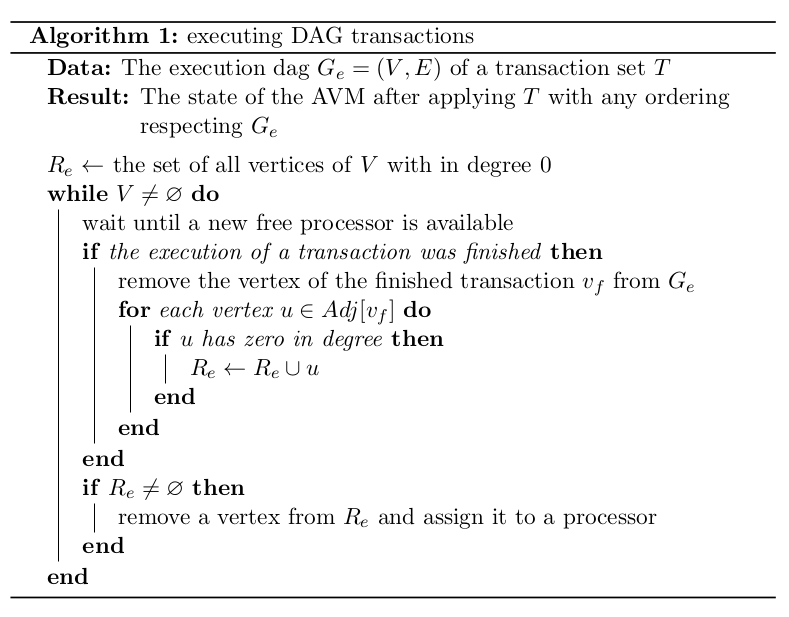
\includegraphics[width=17cm]{../img/Alg1s.png}
\begin{algorithm}[t]
    \DontPrintSemicolon
    \SetKwInOut{Input}{input}\SetKwInOut{Output}{output}
    \Input{A sequence of $n$ digits in base $\beta$: $d_{1}d_{2}\dots d_{n}$ \newline
    A prefix tree: $<A^{(1)},A^{(2)},A^{(3)},\dots>$}
    \BlankLine
    \Output{Valid identifier prefix of the sequence.}
    \BlankLine
    \For{$i = 1$ \KwTo $n$}
    {
        \If{$(0.d_{1}d_{2}\dots d_{i})_\beta < A^{(i)}$}
        {
            \KwRet{$d_{1}d_{2}\dots d_{i}$}\;
        }
    }
    \KwRet{NIL}\;
    \caption{Finding a prefixed identifier}\label{alg:prefix_id}
\end{algorithm}

When we have a prefixed identifier, and we want to know if a sequence of digits is marked by that identifier,
we use Algorithm~\ref{alg:match_id} to match the prefixed identifier with the start of the sequence. The matching
can be done with only three comparisons, and an invalid prefixed identifier can be detected and will not match
any sequence.

In Argennon the shorter prefix codes are assigned to more active accounts and smart contracts which tend to own more
data objects in the system. The prefix trees are designed by analyzing empirical data to make sure the number
of leaves in each level is chosen appropriately.

\begin{algorithm}[h]
    \DontPrintSemicolon
    \SetKwData{Id}{$id$}
    \SetKwInOut{Input}{input}\SetKwInOut{Output}{output}
    \Input{A prefixed identifier in base $\beta$ with $n$ digits: $\Id=a_{1}a_{2}\dots a_{n}$ \newline
    A sequence of digits in base $\beta$: $d_{1}d_{2}d_{3}\dots $ \newline
    A prefix tree: $<0,A^{(1)},A^{(2)},A^{(3)},\dots>$
    }
    \BlankLine
    \Output{$TURE$ if and only if the identifier is valid and the sequence starts with the identifier.}
    \BlankLine
    \If{$(0.a_{1}\dots a_{n})_\beta = (0.d_{1}\dots d_{n})_\beta$}
    {
        \If{$A^{(n-1)} \leq (0.a_{1}a_{2}\dots a_{n})_\beta < A^{(n)}$}
        {
            \KwRet{TRUE}\;
        }
    }
    \KwRet{FALSE}\;
    \caption{Matching a prefixed identifier}\label{alg:match_id}
\end{algorithm}


\section{Heap Chunks}\label{heap}

The persistent data of an Argennon application is stored in heap chunks. An application may have several heap chunks
with different sizes, and can remove or
resize its chunks or allocate new chunks. Every chunk belongs to exactly one application. Only the owner application can
modify a chunk but there is no restrictions for reading a chunk.

When an application allocates a new heap chunk, the identifier of the new chunk is not generated by
the AscEE. Instead, the application can choose an identifier itself \footnote{provided it has a correct format}. This
is an important feature of the AscEE's heap, which allows applications to use the AscEE's heap as a dictionary (map)
data structure.
Since the \texttt{chunkID} is a prefix code, any application has its own identifier space, and an application
can easily generate unique identifiers for its chunks.

A heap chunk can be considered as a continuous
array of bytes. Every chunk has a size: \texttt{chunkSize} and a size upper bound: \texttt{sizeUpperBound}. The value of
\texttt{chunkSize} can be determined uniquely at
the start of
every execution session, and it may be updated during the session like a normal memory location. On the other hand,
the value of \texttt{sizeUpperBound} is constant for every block of the blockchain and is proposed by the block
proposer.

The address space of a chunk starts from zero and only offsets lower than \texttt{sizeUpperBound} are valid. Trying to
access any offset higher than this value will result in a revert for the application.

\subsection{Access Blocks}\label{subsec:access-blocks}

Memory locations inside a chunk can only be accessed through access blocks. An access block is defined on a chunk
and has an offset and a size and determines accessible memory locations inside a chunk. Multiple access blocks can
be defined on a chunk, but they must be non overlapping. Access blocks are byte addressable and can have different
access types:

\begin{itemize}
    \item \texttt{read\_only}: only allows read and check operations.
    \item \texttt{writable} memory locations inside this access block can not be modified.
    \item \texttt{check\_only}: only allows check operations. These operations query the persistence
    status of memory locations.
    \item \texttt{additive}: only allows addition operations without overflow checking. Note that the content of these
    access blocks cannot be read.
\end{itemize}

Chunks are intended for simplifying proof checking of the data stored in the Argennon cloud and access blocks are
required for better parallelization of request execution. An application should put the data it predicts is needed for
validating a block in the same chunk and put the data it predicts will be needed in a single execution session in
the same access block.

\subsection{Chunk Resizing}\label{subsec:ch-resize}

The value of \texttt{chunkSize} at the end of the execution session will determine if a memory location at an
offset is persistent or not: Offsets lower than the chunk size are persistent, and higher offsets are not.
Non-persistent locations will be re-initialized with zero, at the start of every execution session.

The value of chunkSize can be modified during an execution session. However, the new size values can only be
increasing or decreasing. More precisely, if a request declares that it wants to expand (shrink) a chunk, it can only
increase (decrease) the value of chunkSize and any specified value for chunkSize during the execution session, needs
to be greater (smaller) than the previous value of the chunk size. Any request that wants to expand (shrink) a chunk
needs to specify a max size (min size). The value of chunkSize can not be set higher (lower) than this value.

Usually an application should not have any assumption about the content of memory locations that are outside the chunk.
While these locations are zero initialized at the start of every execution session, it should be noted that multiple
invocations of an application may occur in a single execution session, and if one of them modifies a location outside
the chunk, the changes can be seen by next invocations.

There is no way for an application to query the chunk capacity. As a result, in the view of an application, accessing
offsets higher than chunkSize results in undefined behaviour, while the behaviour is well-defined for validators.
This enables validators to determine the validity of an offset at the start of the block validation in a parallelized
preprocessing phase without executing requests.

While an application can use \texttt{chunkSize} to determine if an offset is persistent or not, that is not
considered a good practice. Reading \texttt{chunkSize} decreases transaction parallelization, and should be avoided.
Instead, applications should use a built-in AscEE's function for checking the persistence status of memory addresses.

An application can load a chunk with a valid prefix identifier even if that chunk does not exist. For a non-existent
chunk the value of \texttt{chunkSize} is always zero.


\section{Resource Management}\label{sec:res-man}

Completing an execution session needs computational resources. The amount of resources used by an execution session
needs to be monitored, otherwise a spammer would be able to easily exhaust the resources of the execution
environment. Resource usage can be measured per session or per application call.

The AscEE has two type of execution sessions: \emph{optimistic} and \emph{monitored}. Resource usage of an optimistic
session is always measured per session and default pre-defined resource caps are used. On the other hand in a monitored
session some resources are measured per application and some
caps are determined dynamically by the request. An optimistic session must always
complete normally but a monitored session is allowed to either complete normally or abruptly.

Obviously resource monitoring is easier for optimistic sessions, and they can be executed more efficiently. However, if
an optimistic session violates its resource caps, determining the point of failure requires precise resource
measurement. Note that for implementing optional decoupling principle, we need to determine the exact application
which has failed in the call chain. For example assume that an optimistic session containing an application call
violates a 2 milliseconds execution time cap. If in the caller application the call happens exactly after 2
milliseconds of execution, a small fluctuation in the execution time measurement can
change the point of failure between the called and the main application. This will introduce nondeterministic
behaviour which makes block validation impossible. On the other hand, for a monitored session this is not an issue
because resource measurements and caps are defined per application, and we make sure that resource caps are not too
small for any application call.

Different computational resources are measured and monitored during an AscEE session:
\begin{itemize}
    \item \textbf{execution time}:
    the amount of cpu time that is required for executing a session or an application. The execution time of a session
    is measured in \emph{AscEE clocks}. One AscEE clock is defined as 1/1000 of the amount
    of cpu time needed for executing a predefined standard application which is used for benchmarking a host's
    performance.

    Optimistic sessions have a predefined \texttt{maxClocks} value which is determined by the Argennon protocol. This
    value defines a bound on the total cpu time of the session and no per application measurement is done.

    Monitored sessions perform per application cpu-time measurement, and every application call during a monitored
    session has a separate \texttt{maxClocks} value. This value determines the maximum amount of time that the cpu
    can be used for executing that particular application call. It should be noted that the timer is paused when an
    application makes a call to another application, until the control returns to the caller. An application call
    needs at least 100 clocks and if the value of its \texttt{maxClock} is lower than this value the call will be
    considered a failed call.

    Each application call has some amount of \texttt{externalClocks}. When an application makes a request to another
    application it has to \emph{forward} a portion of its external clocks to the called application. This amount
    will determine the value of maxClocks for the called application.

    The amount of external clocks for every application
    call is defined to be \(2/3\) of its \texttt{maxClocks}. As a result the total number of clocks of a monitored
    session is always less than \(3 \times \texttt{maxClocks}\) of the root application. The value of
    \texttt{maxClocks} for
    the root application call is determined by the transaction.

    \item \textbf{local memory}:
    any memory usage of an application that is not part of the heap chunks and is not part of another resource
    will be considered as local memory usage. This resource is measured in bytes.
    \item \textbf{heap access list}:
    every session can only access heap locations that are declared in its access list. In addition,
    resizing heap chunks can only be done in the range of the pre-declared lower bound and upper bound.
    \item \textbf{applications list}:
    a session may only make requests to applications that are declared in its application list.
    \item \textbf{call depth}:
    the number of nested application calls can not be more than a threshold. This threshold is determined by the
    Argennon protocol.
    \item active differed calls:
    \item virtual signatures:
    \item number of locks

\end{itemize}


\section{Arithmetics}\label{sec:arithmetics}

The Argennon Virtual Machine supports signed integer and signed floating point operations. The Argennon Virtual
Machine does not support any type of unsigned arithmetics. All arithmetic operations in the Argennon Virtual Machine
are checked and any type of overflow or underflow will cause a catchable exception to be thrown.


\section{Reentrancy Protection}\label{sec:reentrancy}

The Argennon Virtual Machine provides low level reentrancy protection by defining a dedicated
instruction: \texttt{enter}. When a smart contract executes the \texttt{enter} instruction, it
can not execute that instruction again as long
as the method executing the instruction completes (abruptly or normally). If a smart contract tries to execute
the \texttt{enter} instruction while the method executing that instruction for the first time has not yet completed,
an exception will be thrown.

Smart contracts can completely prevent reentrancy by executing the \texttt{enter} instruction as the first instruction
of their \texttt{dispatcher} method.


\section{Deferred Calls}\label{sec:deferred-calls}


\section{Authorizing Operations}\label{sec:authorizing-operations}

In blockchain applications, we usually need to authorize certain operations. For example, for sending an asset
from a user to another user, first we need to make sure that the sender has authorized this operation. The
Argennon Virtual Machine has no built-in mechanism for authorizing operations, but it provides a rich set of
cryptographic instructions for validating signatures and cryptographic entities. By using these instructions and
passing cryptographic signatures as parameters to methods, a programmer, having users' public keys, can implement
the required logic for authorizing any operation.

\note{Authorization by explicit signatures eliminates the need for approval methods or call back patterns.}

In addition to cryptographic signatures, the Argennon Virtual Machine provides instructions that enable
smart contracts to issue \emph{virtual signatures}. A smart contract can virtually sign a message for a target
smart contract by \texttt{v\_sign} instruction. When a smart contract
virtually signs a message for a target, that message is stored in the internal memory of the AVM, associated with
its signer and the target. The application that is the target of the signature can verify the message
by \texttt{v\_verify} instruction. After verifying the signature, it will be removed from the AVM's internal memory
to make sure a signature will not be used multiple times. The virtual signatures stored in the AVM's internal memory
last for one execution session.

\note{The Argennon virtual machine has no instructions for issuing cryptographic signatures.}


\section{The Argennon Standard Library}\label{sec:asl}

As we explained in Section~\ref{subsec:method-invocation} by using \texttt{invoke\_internal} instruction, a smart
contract can invoke methods of another smart contract in its own context. AVM smart contracts use this instruction to
invoke methods of the AVM standard library. Methods of the AVM standard library are stored
with the \texttt{applicationID} zero in the AVM method area. This implies that the AVM standard library is actually
a part of the root smart contract.

In Argennon, the root smart contract is an updatable smart contract, which can be updated by the Argennon governance
system. This means that bugs or security vulnerabilities in the AVM standard library could be quickly patched and
smart contracts could benefit from bugfixes and improvements of the AVM standard library even if they are
non-updatable. Many important and useful functionalities,
such as fungible and non-fungible assets, access control mechanisms,
and general purpose DAOs are implemented in the Argennon standard library.

All Argennon standards, for instance ARC standard series, which defines standards regarding transferable assets,
are defined based on how a contract should use the AVM standard library. As a result, Argennon standards are
different from conventional blockchain standards. Argennon standards define some type of standard logic and
behaviour for a smart contract, not only a set of method signatures. This enables users to expect certain type
of behaviour from a contract which complies with an Argennon standard.
